\documentclass{article}
\usepackage{amsmath}
\usepackage{graphicx}
\usepackage{enumitem}
\usepackage {amsfonts}
\usepackage{float}
\usepackage{gensymb}
\title{Trigonometry}
\date{}

\begin{document}

\maketitle

\begin{enumerate}
    \item A man observes a car from the top of a tower, which is moving towards the tower with a uniform speed. If the angle of depression of the car changes from $30\degree$ to $45\degree$ in 12 minutes, find the time taken by the car now to reach the tower.
\end{enumerate}

\begin{center}
\textbf{TRIANGLES}
\end{center}

\begin{enumerate}
    \item Construct a triangle $ABC$ with side $BC = 7\, \text{cm}$, $\angle B = 45\degree$, and $\angle A = 105\degree$. Then construct another triangle whose sides are $\frac{3}{4}$ times the corresponding sides of the $\triangle ABC$.
\end{enumerate}

\begin{center}
\textbf{LINEAR}
\end{center}

\begin{enumerate}
    \item A train covers a distance of $300$ km at a uniform speed. If the speed of the train is increased by $5$ km/hour, it takes 2 hours less in the journey. Find the original speed of the train.
\end{enumerate}

\begin{center}
\textbf{ARITHMETIC PROGRESSIONS}
\end{center}

\begin{enumerate}
    \item If the $10^\text{th}$ term of an arithmetic progression (A.P.) is $52$ and the $17^\text{th}$ term is $20$ more than the $13^\text{th}$ term, find the A.P.
    \item If the ratio of the sum of the first $n$ terms of two A.P.s is $\frac{7n + 1}{4n + 27}$, then find the ratio of their $9^\text{th}$ terms.
\end{enumerate}

\begin{center}
\textbf{COORDINATE GEOMETRY}
\end{center}

If the points $A(k + 1, 2k)$, $B(3k, 2k + 3)$, and $C(5k - 1, 5k)$ are collinear, then find the value of $K$.

\begin{center}
\textbf{QUADRATIC EQUATION}
\end{center}

If the roots of the equation $(c^2 - ab)x^2 - 2(a^2 - bc)x + b^2 - ac = 0$ in $x$ are equal, then show that either $a = 0$ or $a^3 + b^3 + c^3 = 3abc$.

\begin{center}
\textbf{RATIONAL FRACTIONS}
\end{center}

\begin{enumerate}
    \item Solve for $x$: 
    \[
    \frac{1}{2x - 3} + \frac{1}{x - 5} = 1 \frac{1}{9},\quad x \neq \frac{3}{2}, 5
    \]
\end{enumerate}

\begin{center}
\textbf{PROBABILITY}
\end{center}

\begin{enumerate}
    \item A bag contains $15$ white balls and some black balls. If the probability of drawing a black ball from the bag is thrice that of drawing a white ball, find the number of black balls in the bag.
    \item Two different dice are thrown together. Find the probability that the numbers obtained have:
    \begin{enumerate}[label=\roman*.]
        \item an even sum, and
        \item an even product.
    \end{enumerate}
\end{enumerate}

\begin{center}
\textbf{SURFACE AREAS AND VOLUMES}
\end{center}

\begin{enumerate}
    \item From a solid right circular cylinder of height $2.4$ cm and radius $0.7$ cm, a right circular cone of the same height and same radius is cut out. Find the total surface area of the remaining solid.
    \item In a rain-water harvesting system, the rain-water from a roof of $22\,\text{m} \times 20\,\text{m}$ drains into a cylindrical tank having a diameter of base $2$ m and height $43.5$ m. If the tank is full, find the rainfall in cm. Write your views on water conservation.
    \item Three semicircles each of diameter $3$ cm, a circle of diameter $4.5$ cm, and a semicircle of radius $4.5$ cm are drawn in the given figure. Find the area of the shaded region.
        \begin{figure}[h!]
            \centering
            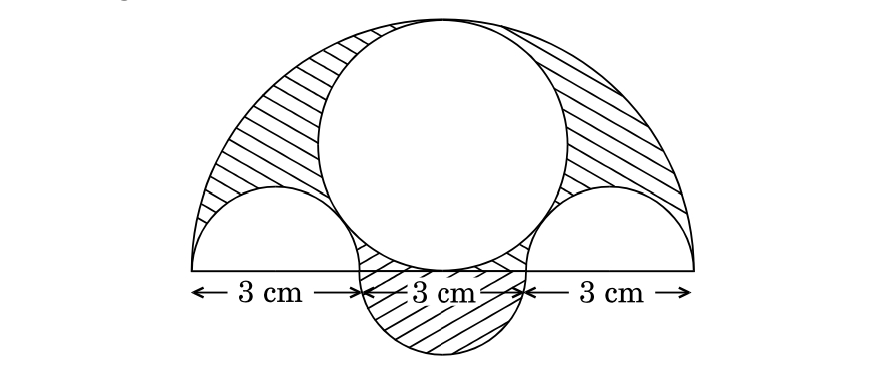
\includegraphics[width=\columnwidth]{areas.jpg}
        \end{figure}
\end{enumerate}

\begin{center}
\textbf{CIRCLES}
\end{center}

\begin{enumerate}
    \item In the given figure, $XY$ and $X'Y'$ are two parallel tangents to a circle with center $O$ and another tangent $AB$ with point of contact $C$, intersecting $XY$ at $A$ and $X'Y'$ at $B$. Prove that $\angle AOB = 90\degree$.\\
    \begin{figure}[h!]
        \centering
        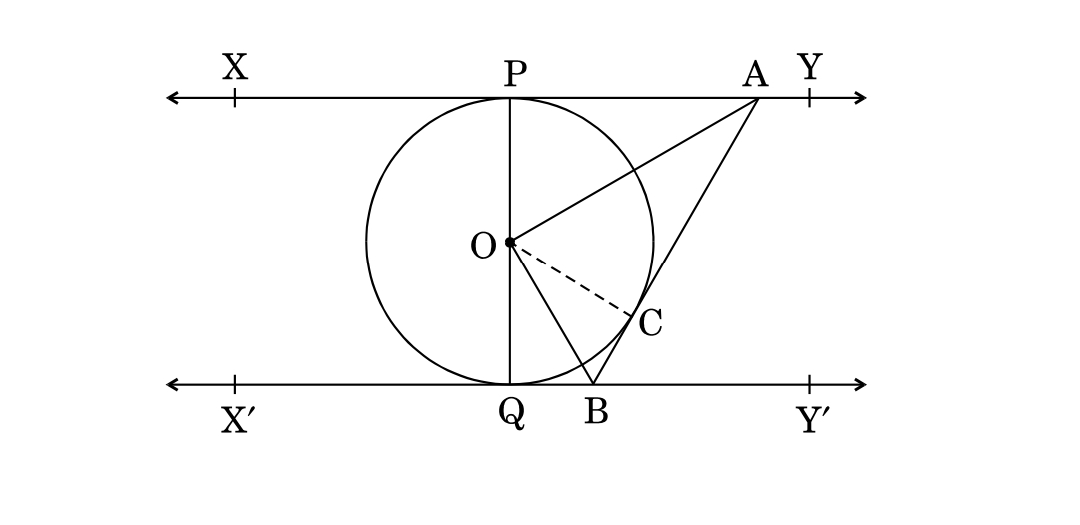
\includegraphics[width=\columnwidth]{circle.jpg}
    \end{figure}
\end{enumerate}

\begin{center}
\textbf{MENSURATION}
\end{center}

\begin{enumerate}
    \item In the given figure, $\triangle ABC$ is a right-angled triangle in which $\angle A = 90\degree$. Semicircles are drawn on $AB$, $AC$, and $BC$ as diameters. Find the area of the shaded region.
    \begin{figure}[h!]
        \centering
        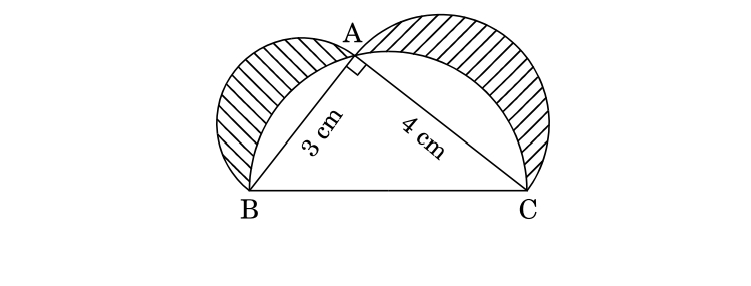
\includegraphics[width=\columnwidth]{mensuration.jpg}
    \end{figure}
\end{enumerate}
i
\end{document}

